% THIS IS SIGPROC-SP.TEX - VERSION 3.1
% WORKS WITH V3.2SP OF ACM_PROC_ARTICLE-SP.CLS
% APRIL 2009

\documentclass{sig-alternate}
% \usepackage{algorithmic}
\usepackage[ruled,lined]{algorithm2e}
\usepackage{tabularx}
\usepackage{graphicx}
\usepackage{graphicx}
\usepackage{stfloats}
\usepackage{multirow}
\usepackage{multicol}
\usepackage{array}
\usepackage{subfigure}
\usepackage{epstopdf}
\usepackage{url}
\usepackage{amssymb,amsmath}
\usepackage{flushend}
\usepackage{microtype} % Margin kerning / font expansion
\usepackage{mathptmx} % Narrow font, designed for multiple columns
\usepackage{enumerate} % enable enumerate[1.]

% \newtheorem{algorithm}{Algorithm}
\newtheorem{definition}{Definition}
\newtheorem{theorem}{Theorem}


\usepackage{etoolbox}
\makeatletter
\patchcmd{\maketitle}{\@copyrightspace}{}{}{}
\makeatother

\begin{document}

\title{Capital Crunch: Predicting Investments in Tech Companies}

% \numberofauthors{1} %  in this sample file, there are a *total*
% % of EIGHT authors. SIX appear on the 'first-page' (for formatting
% % reasons) and the remaining 	two appear in the \additionalauthors section.
% %
\author{
% 1st. author
\alignauthor
Zifei Shan, Haowen Cao and Qianying Lin\\
        \affaddr{Department of Computer Science, Stanford University}\\
        \email{\url{{zifei, caohw, qlin1}@stanford.edu}}
}
% \alignauthor
% Anonymous Author\\
%         \affaddr{Affiliation Line 1}\\
%         \affaddr{Affiliation Line 2}\\        
%         \email{Email}
% }
% 2nd. author
% \alignauthor
% G.K.M. Tobin\titlenote{The secretary disavows
% any knowledge of this author's actions.}\\
%       \affaddr{Institute for Clarity in Documentation}\\
%       \affaddr{P.O. Box 1212}\\
%       \affaddr{Dublin, Ohio 43017-6221}\\
%       \email{webmaster@marysville-ohio.com}

\maketitle

% % A category with the (minimum) three required fields
% \category{H.4}{Information Systems Applications}{Miscellaneous}
% %A category including the fourth, optional field follows...
% \category{D.2.8}{Software Engineering}{Metrics}[complexity measures, performance measures]

% \category{J.4}{Computer Applications}{Social and Behavioral Sciences}
% \category{H.3.5}{Information Storage and Retrieval}{Online Information Services}

% \terms{Security, Design, Experimentation}

\begin{abstract}

For many start-ups, lack of investment and capital has become the
bottleneck for development. This phenomenon inspires us to use machine
learning algorithms to find patterns in investment behavior from major
investors. We propose to use various domain-specific features to predict
which investors would potentially invest in a particular company.
This would not only reveal important information about investment
strategies and behaviors of investors, but also give startups ideas on
where to seek potential investment and how to adjust their strategies
so as to attract potential investors.

Our work is grounded in CrunchBase, an accessible knowledge base that
maintains full records of company and people information.

There are two primary goals of our work:

(1) To predict whether an investor would invest in a particular start-up
based on textual, topological and domain-specific signals from both
the investor and start-up.

(2) To analyze and reveal the factors that would prompt an investor to
invest in startups so as to shed light on the adjustments the start-
ups could make to attract more investments.

\end{abstract}

\keywords
{Machine Learning, Data Mining, Link Prediction, Startups}

\section{Dataset}\label{dataset}

We use data from \emph{CrunchBase.com}, one of the biggest databases
about information of companies. The current CrunchBase dataset includes
214,290 companies and 286,659 people.

\subsection{Accessing data}\label{accessing-data}

CrunchBase provides indexing data and an API for full access of their
data, yet the API has limited throughput. Due to the limitation, by now
we would like to sub-sample the dataset, and we may get the full dataset
in the future.

For data sub-sampling, a possible strategy is random sampling. However,
it would have the potential drawback that we might not achieve
consistency amongst different parties. (e.g.~Facebook is sampled but its
CEO Mark Zuckerberg is not). Therefore we propose to adopt the strategy
where we start with a ``seed set'' of companies, and iteratively sample
all related people and organizations to grow the network.

\subsection{Data format}\label{data-format}

The detailed data format for people and companies is demonstrated below.

\small

\begin{verbatim}
// people                  // company
"data": {                  "data": {           
  "uuid": "a01b8d...",      "uuid": "770db0...",                         
  "properties": {            "properties": {                   
    "bio": ...                 "description": {...}                
    "last_name": ...           "founded_on": {...}                      
    "first_name": ...          "name": {...}                       
    ...                        "number_of_employees": {...}
  }                          }     
  "relationship": {          "relationships": {...}                     
    "degrees": {...}         "board_members_and_advisors": {...}
    "experiences": {...}     "acquisitions": {...}                          
    "news": {...}            "competitors": {...}                   
    ...                      ...         
  }                        }     
}                          
\end{verbatim}

\normalsize

\section{Proposed Approach}\label{proposed-approach}

\subsection{Data Model}\label{data-model}

The CrunchBase dataset has a variety of entities: organization, person,
product, etc. There are also different relations including investment,
acquisition, degree, founder, etc.

For simplification, we categorize organizations into \textbf{startups}
and \textbf{investors}, and we care about predicting \textbf{investment}
relationship between them.

The data model is defined below:

\begin{itemize}
\itemsep1pt\parskip0pt\parsep0pt
\item
  \(Startup(startupId, [attributes...])\)
\item
  \(Investor(investorId, [attributes...])\)
\item
  \(Investment(investorId, startupId, isTrue)\)
\end{itemize}

Where we use features in \(Startup\) and \(Investor\) entities to
predict \(Investment\) relations.

\subsection{Problem definition}\label{problem-definition}

Our former problem is:

\begin{definition}\label{def:problem}

Problem: given the full \textbf{Startup} relation and
\textbf{Investor} relation, predict \textbf{isTrue} value in
\textbf{Investment} table, which determines if any given investor
invests a startup.

\end{definition}

\textbf{The desired output} is a predicted probability between each
investor and a startup. For example:

\small

\begin{verbatim}
# investor  startup         probability
facebook    hello-doctor    0.95
google      hello-doctor    0.85
google      zynga           0.97
twitter     zynga           0.45
\end{verbatim}

\normalsize

\subsection{Features}\label{features}

A rich set of features can be applied to predict investments. They may
include:

\begin{itemize}
\itemsep1pt\parskip0pt\parsep0pt
\item
  Company attributes. e.g.~date founded, number of employees.
\item
  Attributes of correlated people. e.g.~degrees of founders and
  employees.
\item
  Linguistic features: information buried in company descriptions and
  biography of people.
\item
  Network topology, e.g.~make use of all relations including degree,
  founder and other investments. These feature may be only captured by a
  factor graph model discussed later.
\end{itemize}

\subsection{Model}\label{model}

A naive baseline model would be a random predictor that predict random
labels based on some class priors. An oracle would be one that knows all
existing investments and give correct predictions.

Our initial model would be training an independent logistic regressor
for each individual investor, that takes a feature vector of a start- up
and predicts a label. The drawback of this model is that it can hardly
utilize investor-based attributes and higher-level knowledge such as
network topology.

As an improvement, we propose to apply a factor graph model that
correlates features across this graph. Specifically, each \(Investment\)
relation is a boolean variable that we are predicting, and features in
both sides of investors and startups can be correlated. We can further
design features for more complex correlations.

\subsection{Getting training data}\label{getting-training-data}

To train the predictor, we take ground truth investments in CrunchBase
as positive training examples, that is, if an investor \(I\) has
invested in a startup \(S\), we obtain a training example
\((I, S, true)\) in \(Investment\) relation.

For the negative training examples, it might not be desirable to simply
label all pairs of \((investor, startup)\) that do not have a known
investment as negative, because (1) this makes positive examples
extremely sparse and introduce a data skew, and (2) even if an investor
have not invested a startup right now, it is still possible that the
invest will happen in the future. How to effectively label negative
examples is still open to us. For now we propose to take random pairs of
investors and startups with no known investment happening.

\section{Evaluation}\label{evaluation}

We will evaluate our models based on ground truth investments.
Specifically, we hold out a fraction of training examples, and predict
these relations and get measures including precision and recall. We may
want to define our own measure to encourage aggressive predictions and
punish false negatives more than false positives.

Another measure to try is the accuracy of top-K prediction: we hope to
get a trained system where the most confident predictions are very
likely to be true.

An further evaluation method is the calibration plot where we layout the
predicted probabilities and the accuracy in testingset in buckets. See
Figure \ref{fig:calibration}. A discussion of interpreting calibration
plots is in the paper \cite{zhang2014feature}.

\begin{figure}[ht!]
\centering
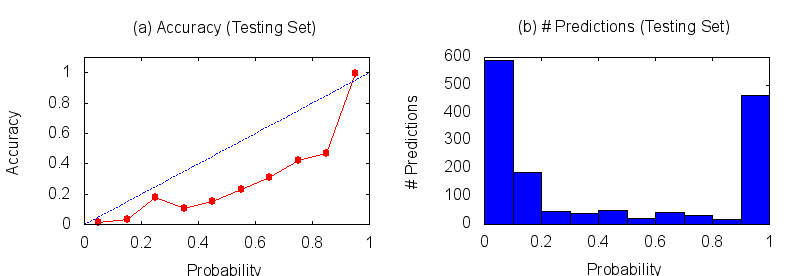
\includegraphics[width=0.4\textwidth]{img/calibration.png}
\caption{A sample calibration plot}
\label{fig:calibration}
\end{figure}

\section{Challenges}\label{challenges}

We see several challenges in the project:

\textbf{Data sparsity.} To predict pairwise investment relationship
between investors and startups, training data might be very sparse and
highly skewed: most investors only invest a few companies. We may reduce
feature space by carefully engineering features through error analysis,
or trying methods like SVD. More advanced models, e.g.~collaborative
filtering, or a joint inference model that correlates prediction on all
investors, would also help tackling the sparsity issue.

\textbf{Feature extraction.} Designing and extracting features are the
key to a successful predictor. To fully utilize the information hidden
from raw text such as company descriptions and founder bios, we propose
to adopt state-of-the-art natural language processing methods for
feature extraction, including named entity recognition and dependency
parse.

\textbf{Model high-level knowledge.} Some high-level knowledge would be
hard to capture by a simple logistic regression model. We propose to use
factor graphs to model the correlations between different investors,
company and people, etc.

\textbf{Scalability.} If we are building a factor graph model with a
large feature space, it would be hard to do learning and inference on
the graph. We propose to use DeepDive \cite{zhang2014feature}, a highly
scalable inference engine to tackle the problem.

\textbf{Future extensions.} If time permits, we might extend our model
to predict company acquisition in this dataset. We also propose to do
analysis on important factors in investment and acquisition behaviors.

\section{Related Work}\label{related-work}

In the paper \cite{an2014recommending}, the author discussed a
methodology to match proposals from start-ups to the potential investors
on Kickstarter with linear regression, SVM-linear, SVM-poly and SVM-RBF,
with an accuracy rate of 82\% for static data features and 73\% for
dynamic data features. Their features are mostly updates made to the
tweets, number of comments and so on, and we could widely expand the
feature set.

Another paper \cite{gartner1999predicting} used a discriminant analysis
to classify the potentially successful and unsuccessful companies. Their
feature sets are worth noting, including individual characteristics of
the entrepreneurs, the efforts by entrepreneurs (i.e.~whether they
actively look for resources and help), degree of innovation and so on.
Though this paper is more on the social science side, we would like to
scrutinize the feature sets so as to explore more meaningful and
insightful features. For example, we could extend individual
characteristics to how many start-ups the CEO has founded and their
histories.


% \section*{Acknowledgment}

\bibliographystyle{abbrv}
\bibliography{src/cs221}

\end{document}
